\chapter*{About the author}
\addcontentsline{toc}{chapter}{About the author}

\begin{wrapfigure}{r}{0.5\textwidth}
    \vspace{-20pt}
    \begin{center}
        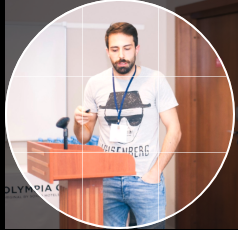
\includegraphics[width=0.48\textwidth]{images/me_linkedin}
    \end{center}
    %\vspace{-20pt}
    %\caption{A gull}
    \vspace{-15pt}
  \end{wrapfigure}

Davide Spataro was born in 1990 and grew up in Nicotera, a small but beautiful city by the Tyrrhenian Sea in Southern Italy. 
He own a Ph.D. in Mathematics and Computer science and his main research interests revolved around the central topic of \textit{Parallel Computing} and \textit{GPGPU} in the context of High-Performance Computing (HPC) for the simulation of macroscopic natural phenomena like landslides. 

In 2011, he obtained the Bachelor of Science in Computer Science at the University of Calabria. and since 2014 he holds the Master of Science (summa cum laude).
Since April 2015 member of the NVIDIA GPU Educational Center at UNICAL.
In  January 2018 he succesfully defended his Ph.D. thesis with title: \textit{Acceleration of numerical regular grid methods on manycore systems}. From 2018 to 2020 he worked as Software Design Enginner at ASML on the next generation of Extreme Ultraviolet lithography machines.
From 2020 he is a Senior Software Engineer at DEGIRO. 


He is a curious and passionate software engineer, an active StackOverflow user and an avid reader of technical and scientific books and articles.
He regularly participates in competitive programming competitions, writes articles on C++ and algorithms and gives computer science online lesson. 
Besides that, I am passionate about
cycling, photography and investing.

When he is  not coding, he is most likely either
paddling in the Mediterranean sea,
lifting weights in the gym or fighting
gravity on a race bike. 
He drinks a lot of
coffee. 
